% Document class / Dokumentenklasse:
\documentclass{LNTthesis}
% Parameters of the LNTthesis class:
% DIV12       = document layout: DIV factor = 12 (larger number creates larger pages)
% BCOR12mm    = binding correction: 12mm
% headsepline = separate page head by a line
% twoside     = twosided document
% 11pt        = font size 11 point
% openright   = start new chapters only on right pages (odd numbered pages)
% more information: http://tug.ctan.org/tex-archive/macros/latex/contrib/koma-script/scrguien.pdf

% Packages used in LNTthesis class:
% package[english]{babel}   % english language / Englische Sprache
% package{LNTthesis}        % LNT specific definitions / LNT spezifische Definitionen
% package{graphicx}         % for using eps images / Einbinden von EPS Grafiken
% package{verbatim}         % for quickly commenting out large parts of your text / Um viel Text schnell auskommentieren zu koennen
% package{amssymb}          % additional math symbols / Zusaetzliche mathematische Symbole
% package{amsmath}          % additional math commands / Zusaetzliche mathematische Befehle
% package{amsxtra}          % even more math symbols / Noch mehr mathematische Symbole
% package{amsthm}           % theorem environment etc / Theorem Umgebung usw
% more information on amsmath: http://www.ctan.org/get/macros/latex/required/amslatex/math/amsldoc.pdf

% package{psfrag}           % psfrag: http://www.ctan.org/get/macros/latex/contrib/psfrag/pfgguide.pdf
% package{subfigure}        % enable subfigures / Ermoeglicht Subfigures (mehrere Figures neben/untereinander)

% !! PLEASE READ THE LATEX HELP IF YOU HAVE ANY QUESTIONS !!
% http://tobi.oetiker.ch/lshort/lshort.pdf


% Macros:
    \newcommand{\eq}[1]{Equation (\ref{#1})}        % \eg{eq:golomb}  --> Equation (2.15)
    \newcommand{\eref}[1]{(\ref{#1})}               % \eg{eq:golomb}  --> (2.15)
    \newcommand{\fig}[1]{Figure \ref{#1}}           % \fig{fig:golomb}--> Figure 2.15
    \newcommand{\tab}[1]{Table \ref{#1}}            % \tab{tab:lala}  --> Table 2.15
    \newtheorem{prop}{Proposition}

% Abbreviations
    \newcommand{\equivalent}{\triangleq}
    \newcommand{\given}{\:\!\vert\:\!}


% Document:
\begin{document}

% ###################################
% Title page / Titelseite
% ###################################
\LNTtitle{Master's Thesis}          % Thesis type / Art der Arbeit (Master's Thesis, Diplomarbeit)
    {Software implementation of Polar codec for 5G}                  % Thesis title / Titel der Arbeit
    {Yadhunandana Rajathadripura Kumaraiah}                  % Your name / Name des Diplomanden
    {Dipl.-Ing.~Advisor}            % Advisor / Betreuer
    {M\"unchen, Month Year}          % Munich, Date / Muenchen, Datum
    {Yadhunandana Rajathadripura Kumaraiah\\                 % Your Address / Anschrift des Diplomanden
    Schr\"ofelhofstra\ss e 14 WG 02/02\\
    81375 M\"unchen\\
    yadhu.kumaraiah@tum.de}

\LNTrecht{Yadhunandana Rajathadripura Kumaraiah}             % Your name / Name des Studenten
    {M\"unchen, xx.xx.20xx}         % Munich, Date / Muenchen, Datum

\cleardoubleemptypage   % start new double page / neue Doppelseite

% ########################################
% Table of Contents / Inhaltsverzeichnis
% ########################################

% roman page numbering, starting with page number 1 / roemische Seitennummerierung beginnend mit Seite 1
    \setcounter{page}{1}
    \pagenumbering{roman}

        \tableofcontents    % Table of contents / Inhaltsverzeichnis
        \listoffigures      % List of figures / Abbildungsverzeichnis
        \listoftables       % List of tables / Tabellenverzeichnis
        \cleardoubleemptypage   % start new double page / neue Doppelseite

% ########################################
% Chapters / Kapitel:
% ########################################

% arabic page numbering, starting with page number 1 / arabische Seitennummerierung beginnend mit Seite 1
    \setcounter{page}{1}
    \pagenumbering{arabic}

        %%%%%%%%%%%%%%%%%%%
\chapter*{Abstract}
%%%%%%%%%%%%%%%%%%%
Software implementation of error correction and signal processing applications on general purpose processors has gained interest in recent times. Mainly due to latest technological developments in general purpose computing world. Implementations in software have an inherent advantage not being tied to one specific hardware architecture. They require much less development and maintenance effort compared hardware implementations. For the device manufacturer software implementation provides platform flexibility in addition to reducing the cost of product. \newline

In this thesis, we study the feasibility of developing complete polar FEC chain of $5^{th}$ generation cellular mobile communication standard in software. Specifically on general purpose processors. Thesis work attempts to achieve stringent latency requirements through software, algorithmic and platform specific optimizations. Many algorithms in FEC chain are optimized for hardware implementations. Direct implementation of these algorithms in software results in poor performance. To obtain best performance on general purpose processors these algorithms are modified or reformulated to suit software implementation. Initially both encoding and decoding FEC chain are implemented functionally without any algorithm reformulation or optimization. Code profiling is performed on this naive implementation to identify the significant latency contributors. We split algorithms of significant latency contributing components into primitive operations. These primitive operations are mapped to specialized functional units of general purpose processor to achieve best performance. \newline

We concentrate on polar encoding and decoding FEC chain which are used transmitting control information. Latency contributing components are identified. Algorithms of those components are reformulated to avoid or to reduce latency contributing operations. Major latency contributors in encoding FEC chain were Cyclic redundancy check (CRC) calculation, polar code construction, polar encoding. In decoding FEC chain  subblock deinterleaver, polar decoder, parity bit extraction, CRC calculation. Algorithms of these components are reformulated to suit software requirements and implemented using efficient \emph{vector processing instruction sets}. Algorithms are modified to reduce complexity and lookup tables are used to avoid complex computations. Other optimizations include function unrolling, avoiding superfluous copy operations, hints to compiler for better instruction scheduling and block wise copying et cetera. At the end of both encoding and decoding chapter latency comparisons between naive and optimization are presented. In decoding FEC chain chapter, latencies of decoder of this work and state of the art decoder are compared.     % Include abstract / Einbinden von Kurzfassung und Abstract
        %%%%%%%%%%%%%%%%%%%%%%%%%%%%%%%%%%%%%%%%%%%%%%%
\chapter{Introduction and Motivation} \label{chap:introduction}
%%%%%%%%%%%%%%%%%%%%%%%%%%%%%%%%%%%%%%%%%%%%%%%



In 1948, scientists at the Bell Laboratories achieved two landmark research results:
Claude E.~Shannon published his paper \emph{A mathematical theory of communication} and John Bardeen, Walter Brattain and William Shockley announced the invention of the \emph{transistor effect}.

\cite{Arikan}

A binomial distribution is shown in Figure~\ref{fig:coin_bino}.

\begin{figure}[!htb]
    \centering
    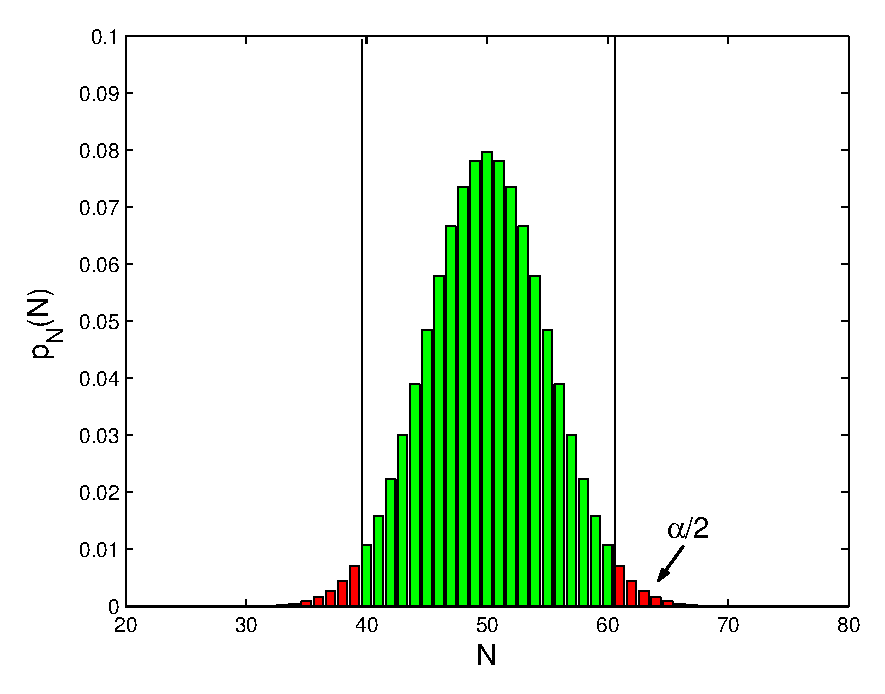
\includegraphics[width=0.8\textwidth]{./figures/coin_bino.eps}
    \caption{PDF $p_N(N)$ of the number N of times that the head side is up.}
    \label{fig:coin_bino}
\end{figure}

For further information, the reader is referred to~\cite{Cover}.\newline

Traditionally FEC chains are developed in hardware i.e FPGA’s or ASIC’s to achieve low latency and high throughput.
Development in FPGA/hardware requires more time and costly.
With recent advances in General Purpose Processors it is possible to achieve required latency and throughput with software implementations without custom hardware.
Software implementations are flexible and easy to maintain compared hardware implementations.

However algorithms need to be adopted/optimized to efficiently implement in software.

Recent advances in the modern processors such as SIMD units can be utilized to achieve low latency and high throughput.



\clearpage
  % Include introduction / Einbinden des Kapitels Einleitung/Problemstellung
        %\include{...}          % Include ... / Einbinden des Kapitels ...
        %\include{simulation}   % Include simulation results / Einbinden des Kapitels Simulation
        \chapter{Conclusion and Outlook} \label{chap:conclusion}
The objective of this work is to study the feasibility of developing polar FEC chain of 5G in software on general-purpose-processor while satisfying stringent latency requirements. In other words, all the components of encoder and decoder FEC chain are developed on general purpose AMD EPYC processor. The software satisfies latency constraint of less than 50$\mu$s. In the first part of the thesis, we provide necessary background about polar encoding/decoding and computer architecture. In the second part, we develop encoding and decoding FEC chains and optimize them to satisfy the necessary latency constraints. \newline

To begin with, we provided necessary mathematical background about polar code construction, polar encoding, and decoding. Including different polar decoding algorithms. To understand FEC chain development in software it is necessary to know the basics of modern computer architecture. Computer architecture section talks about pipelining, cache memory and vector processing units in modern general purpose processors. \newline

In the next chapter, we talk about the details of polar encoding FEC chain. In this chapter, we analyze the different components of the FEC chain to identify latency contributors. Each of these latency contributors is further studied to reformulate the algorithm to avoid costly operations. Algorithms are reformulated to fit into specialized functional units of modern processors such as vector processing units. Vector processing units allow data parallelism in addition to supporting very fast mathematical computations. The encoding,  major latency contributors were polar code construction, CRC calculation, encoding, and rate matching. A wide range of optimization techniques is employed to reduce the latency both algorithmic and platform specific. Namely, reducing algorithm complexity, using lookup tables, compiler hints for better instruction scheduling, vector processing instructions for data parallelism and avoiding superfluous copy operations et cetera. Optimizations reduced the worst-case latency of the encoding FEC chain from $451 \mu$s to $40\mu$s which is more than 10x reduction in latency. \newline

For the decoding FEC chain again same steps as encoding chain are followed to identify the latency contributors. Major contributors in decoding FEC chain were channel deinterleaver, subblock deinterlever, polar decoder, parity bit extractor, and CRC calculation. Decoding FEC chain extensively uses SIMD, bit count, cache prefetching instructions to reduce latency. Subblock deinterleaving operation is divided into three primitive small operations which are implemented efficiently with $\mathtt{permute}$ and $\mathtt{blend}$ vector instructions. The polar decoder is optimized by implementing XOR, CN, VN, bit combination and frozen pattern identification operations using vector processing instructions. Parity bit extractor optimized by avoiding expensive remove and erase operations instead uses modified algorithm marking indexes and dynamically calculating hamming weights of generator matrix rows. Finally, for CRC calculation an algorithm based on lookup table is developed based on \cite{Sarwate:1988:CCR:63030.63037} which processes block of data bits to calculate CRC. These optimizations significantly reduced the latency of decoding FEC chain from $391 \mu$s to $40\mu$s almost a 10x reduction in latency. \newline

As an outlook, for the above stated decoding FEC chain, decoder is developed with \emph{fast-SSC} algorithm. This algorithm has much lower error correction performance than similar block-length LDPC and Turbo counterparts. As part of this work, \emph{CRC-Aided Successive Cancellation List} (\emph{CA-SCL})\cite{SCL} decoding algorithm is also implemented, however, it is not optimized for software. \emph{CA-SCL} ideally suits very low SNR scenarios such as mmWave communication. It has approximately $1.5dB$ gain over \emph{fast-SSC} algorithm for $N=2048$ and list size $L = 8$. Ideal continuation of this work would be to extend the decoding chain by incorporating \emph{CA-SCL} algorithm to the FEC chain. It would be interesting to see the latency values of this algorithm, which has expensive \emph{sort} and \emph{copying} operations.   % Include conclusion/summary / Einbinden des Kapitels Zusammenfassung/Ausblick
        
        \cleardoubleemptypage


% ########################################
% Appendix / Anhang:
% ########################################

% roman page numbering, starting with page number 1 (capitals)/ roemische Seitennummerierung beginnend mit Seite 1 (gross)
    \appendix
    \setcounter{page}{1}
    \pagenumbering{Roman}

        % Use IEEE DIN 1505 style for bibliography / Literaturverzeichnisses
        \bibliographystyle{ieeetransa}
        %\nocite{*}              % Include all references without checking / Alle References immer aufführen
        \bibliography{literature}

\end{document}

%
% EOF!
%